%%%%%%%%%%%%%%%%%%%%%%% file template.tex %%%%%%%%%%%%%%%%%%%%%%%%%
%
% This is a general template file for the LaTeX package SVJour3
% for Springer journals.          Springer Heidelberg 2010/09/16
%
% Copy it to a new file with a new name and use it as the basis
% for your article. Delete % signs as needed.
%
% This template includes a few options for different layouts and
% content for various journals. Please consult a previous issue of
% your journal as needed.
%
%%%%%%%%%%%%%%%%%%%%%%%%%%%%%%%%%%%%%%%%%%%%%%%%%%%%%%%%%%%%%%%%%%%
%
% First comes an example EPS file -- just ignore it and
% proceed on the \documentclass line
% your LaTeX will extract the file if required

\RequirePackage{fix-cm}
\documentclass[smallextended,natbib]{svjour3}       % onecolumn (second format)
\smartqed  % flush right qed marks, e.g. at end of proof
\usepackage{graphicx}
\usepackage{mathptmx}      % use Times fonts if available on your TeX system
%
% insert here the call for the packages your document requires
%\usepackage{latexsym}
% etc.
\usepackage[utf8]{inputenc}
\usepackage[T1]{fontenc}
\usepackage{graphicx}
\usepackage{multirow}
\usepackage{booktabs,tabularx}
\usepackage{setspace}
\usepackage{hyperref}
\usepackage{epstopdf}
\usepackage{lineno}
\usepackage{amsmath}
\linenumbers
\DeclareUnicodeCharacter{0301}{\'{e}}
%
% please place your own definitions here and don't use \def but
% \newcommand{}{}
%
% Insert the name of "your journal" with
\journalname{myjournal}
%
\begin{document}

\title{Learning biological dynamics from spatio-temporal data by Gaussian processes%\thanks{Grants or other notes
%about the article that should go on the front page should be
%placed here. General acknowledgments should be placed at the end of the article.}
}
%\subtitle{Do you have a subtitle?\\ If so, write it here}

\titlerunning{Learning biological dynamics from spatio-temporal data by GP}        % if too long for running head

\author{Lifeng Han         \and
        Second Author %etc.
}

%\authorrunning{Short form of author list} % if too long for running head

\institute{F. Author \at
              first address \\
              Tel.: +123-45-678910\\
              Fax: +123-45-678910\\
              \email{fauthor@example.com}           %  \\
%             \emph{Present address:} of F. Author  %  if needed
           \and
           S. Author \at
              second address
}

\date{Received: date / Accepted: date}
% The correct dates will be entered by the editor


\maketitle

\begin{abstract}
We propose a method of learning biological dynamics from spatio-temporal data by Gaussian processes (GP). This approach is essentially ``equation free'' and hence avoids model derivation, which is often difficult due to high complexity of biological processes. By exploiting the local nature of biological processes, dynamics can be learned in a data efficient manner. With a carefully chosen covariance function, learning reveals key insights of the underlying process and enables propagation uncertainty in multi-step forecasting. The methodology shows promising results when tested on synthetic data. We also demonstrate a case study on real image data of real E. coli colony.  
\keywords{First keyword \and Second keyword \and More}
% \PACS{PACS code1 \and PACS code2 \and more}
% \subclass{MSC code1 \and MSC code2 \and more}
\end{abstract}

\section{Introduction}
\label{intro}
Mathematical models have been used to study biological processes. High complexity of biological systems makes derivation of models from first principle difficult. Oftentimes many assumptions have to be made in the process of model formulation.  It is hard to validate these assumptions. Spatial-temporal biological processes pose a problem of higher dimensionality making resolving the aforementioned issues more challenging. For example, in predicting brain tumor growth, models as simple as one partial differential equation (PDE) \citep{Jackson2015a} and as complicated as a system of PDEs coupled with ordinary differential equations \citep{Eikenberry2009} were used. The mechanism of migration of tumor cells can be modeled as simple as linear diffusion  or as complicated as cell adhesion and repulsion from a mechanic perspective \citep{khain2012migration,aubert2008model}. In clinical settings, an available data set usually consists of a few brain images, which is the only observational data that many models rely on \citep{lipkova2019personalized,Kostelich2011a,Jackson2015a}. Parameter identifiability is of concern as well as the possibility of under or over fitting. In this paper, we propose a purely data-driven approach to forecast biological spatio-temporal processes, which circumvents the aforementioned issues.              

Data-driven model discovery has emerged as a vibrant field that focuses on letting data dictate model formulation instead of basing on superfluous or subjective assumptions \citep{Brunton2019}. There are two popular approaches of data-driven model discovery. One utilizes machine learning techniques or descriptive statistical models which oftentimes offer a black-box solution. This approach does not reveal an explicit model, and hence lacks interpretability or mechanism. The other is based on sparse regression to select terms from an extensive library of model terms. Recent developments on denoising has made it popular in handling noisy biological data \citep{Nardini2020,Lagergren2020a}.

Gaussian processes (GP) regression is a machine learning technique that can be used for model discovery. GP is a type of random function with nice features suitable for Bayesian learning: inference can be made with analytical tractability on the random function given data. Applying to dynamical systems, GP can be used to represent either the state or the transition function of a dynamical system.   Raissi et al \citep{Raissi2018,Raissi2018a} pioneered in unitizing GP to estimate parameters of PDE models and propagate uncertainty.  By representing the system state as GP, it is essentially a mesh-free numerical method and depends on a known PDE formulation. So it does not strictly fall in the category of model discovery. On the other hand, representing transition function as a GP has gained substantial exposure in the literature of machine learning and system identification \citep{girard2003gaussian,deisenroth2009analytic} where it is sometimes called recurrent GP since GP is used recurrently to map one state to the next in time. For example, it has been successfully used to predict pedestrian's movement for self-driving cars \citep{Wang2008}. However, they are motivated by engineering applications and mostly concerned with problems with state space of a small number of dimensions. Applications to biological spatio-temporal processes are unprecedented to our knowledge, which we try to address in this paper.

To learn biological dynamics from spatio-temporal data, we have to overcome the challenge imposed by high dimensionality, which is inevitable due to the necessity to representing space. A continuous state space is usually infinite dimensional. Even if the space is discretized, many grid points are needed to well represent the space. It is challenging to learn the transition function as it is a map on high dimensional spaces. Dynamic mode decomposition, based on singular value decomposition for dimensionality reduction, is a candidate solution to this issue \citep{schmid2010dynamic}. However, it is known to fail if the system demonstrate traveling-wave like solution, which is unfortunately common for biological systems (\citep{Brunton2019} Chapter 6). Another challenge is that biological data is often limited. In spite of being in the era of big data, the small data use cases in biology has risen attention of researchers \citep{Lagergren2020}.  For example, in modeling spatial growth of brain tumor, only a few images of the brain are available, for which it is only feasible to parameterize simplest PDE models \citep{Han2019b,lipkova2019personalized,McDaniel2013}. Indeed, the method in this paper is motivated by the needs to predict brain tumor growth with limited data. The novelty of our method is its data efficiency, which is enhanced by exploiting the local nature of biological spatio-temporal processes (henceforth we name it the local GP method). As a result, the transition function can be effectively learned using only two consecutive data in time. Back to the example of brain tumors, these two consecutive data are usually available as diagnostic and presurgical imaging of the brain tumor. Once the transition function is learned, we can make forecasting onward by recurrently applying it. By exploiting Gaussianity, uncertainty can be propagated with exact integration, which reduces computational costs in contrast to computationally demanding methods that employ ensemble simulation or Monte Carlo sampling \citep{lipkova2019personalized,McDaniel2013}. Furthermore, even though our method does not lead to an explicit model formulation, it determines the size of local neighborhood as a result of training. This key finding reveals time and space scaling of the underlying process, an important insight of a spatial dynamical system.  
               
The paper is organized as the following. In Section \ref{sec:GP-method}, we motivate and describe the local GP method. In Section \ref{sec:syn-data}, we test the method with synthetic data and real image data of E. coli colony. In Section \ref{sec:GP-conclude}, assumptions made in this work are discussed and future directions are pointed out.

\section{Method} \label{sec:GP-method}
We first briefly review the GP regression and introduce notations. More details can be found in \citep{Rasmussen2006}. A GP $f(x)$, denoted as $f\sim\mathcal{GP}(m(x),k(x,x'))$, is a stochastic process that is entirely determined by its mean function $m(x)$ and its covariance function $k(x,x')$. For any finite collection of $x_{i}$ with $i=1\ldots n$, the joint distribution of $f(x_{1}),f(x_{2})\ldots f(x_{n})$ is a multivariate normal with mean $m(x_{1})\ldots m(x_{n})$ and covariance matrix with entry being $k(x_{i},x_{j})$. The GP regression assumes a model $y=f(x)+\epsilon$ where $\epsilon\sim N(0,\sigma^{2})$, and places a GP prior on the latent function $f$, denoted as $f\sim\mathcal{GP}(m(x),k(x,x')$. Given $n$ training data $\mathcal{D}=\{x_{r},y_{r}:r=1\ldots n\}$ where $y_{r}=f(x_{r})+\epsilon_{r}$ as input-output pairs, the GP regression makes inferences of $f(x_{j}^{*})$ at the $m$ test input $x_{j}^{*}$ with $j=1\ldots m$ by conditioning on $\mathcal{D}$. The conditional is easily worked out since the joint distribution is a multivariate normal, i.e., 
\[
\begin{bmatrix}\mathbf{f}\\
\mathbf{f}^{*}
\end{bmatrix}\sim N(\begin{bmatrix}m(\mathbf{x})\\
m(\mathbf{x}^{*})
\end{bmatrix},\begin{bmatrix}\Sigma & K_{*}\\
K_{*}^{T} & K_{**}
\end{bmatrix})
\]
where $\mathbf{f},\mathbf{f}^{*},m(\mathbf{x})$ and $m(\mathbf{x}^{*})$ are vectors, and $\Sigma=k(\mathbf{x},\mathbf{x})+\sigma^{2}I,\ K_{*}=k(\mathbf{x},\mathbf{x}^{*}),\ K_{**}=k(\mathbf{x}^{*},\mathbf{x}^{*})$ are matrices. Here for the ease of notation we have combined individual training data $x_{r},y_{r}$ and and test points $x_{j}^{*}$ into bold notations so that the function acting on them are understood as vectors or matrices. For example, $m(\mathbf{x})$ is a vector with j-th component being $m(x_{j})$ and $k(\mathbf{x},\mathbf{x}^{*})$ is a matrix with entries $[k(\mathbf{x},\mathbf{x}^{*})]_{ij}=k(x_{i},x_{j}^{*})$. As a result, 
\begin{equation}
\mathbf{f}^{*}\vert\mathbf{f}\sim N(m(\mathbf{x}^{*})+K_{*}^{T}\Sigma^{-1}(\mathbf{f}-m(\mathbf{x})),K_{**}-K_{*}^{T}\Sigma^{-1}\Sigma_{*}). \label{eq:f|f*}
\end{equation}
Note that in the standard GP regression, training input $\mathbf{x}$ and testing input $\mathbf{x}^{*}$ are noise-free. In the case of otherwise, the uncertainty in $\mathbf{x}$ and $\mathbf{x}^{*}$ can be taken into account by making appropriate assumptions and approximation. 


We motivate our method by looking at a commonly used PDE model of brain cancer invasion: the Fisher-KPP equation
\[
u_{t}=Du_{xx}+\rho (1-u)u
\]
where $u(x,t)$ is the cancer cell density at position $x$ and time $t$. Finite difference discretization gives 
\[
u_{j}^{n}=u_{j}^{n-1}+\frac{D \Delta t}{\Delta x^{2}}(u_{j+1}^{n-1}-2u_{j}^{n-1}+u_{j-1}^{n-1})+\rho \Delta t u_{j}^{n-1}(1-u_{j}^{n-1}),
\]
where superscripts indicate time and subscripts indicate space. This discretization reflects the local nature of the spatio-temporal process. In fact, there is no well-established governing law of tumor growth. So instead we write a generic transition function $f(\cdot)$ that maps the state variables from time $n-1$ to $n$ and wish to learn it from data. Let $\mathbf{u}\equiv(u_{j})_{j\in\{1:n_{x}\}}$ and we have 
\begin{eqnarray}
\mathbf{u}^{n} & = & f(\mathbf{u}^{n-1})+\epsilon\label{eq:un=00003Df(un-1)}.
\end{eqnarray}
where we assume noise $\epsilon\sim N(0,\sigma_{\epsilon}^{2}I)$. Oftentimes we don't have exact measurement of $u$ but a noisy version of it. For the time being, we assume the exact observation of $\mathbf{u}$ is available.

To avoid the curse of dimensionality, we exploit the local nature by making $f$ a local map (Figure \ref{fig:local map}), i.e., $u_{j}^{n}=f(u_{\mathcal{N}(j)}^{n-1})$ where $\mathcal{N}(j$) is an ordered set of local neighbors of $j$ including $j$, and accordingly $u_{\mathcal{N}(j)}^{n-1}$ is a vector with elements $u_{i}^{n-1}$ for $i\in\mathcal{N}(j)$ that preserve this order.

\begin{figure}
\centerline{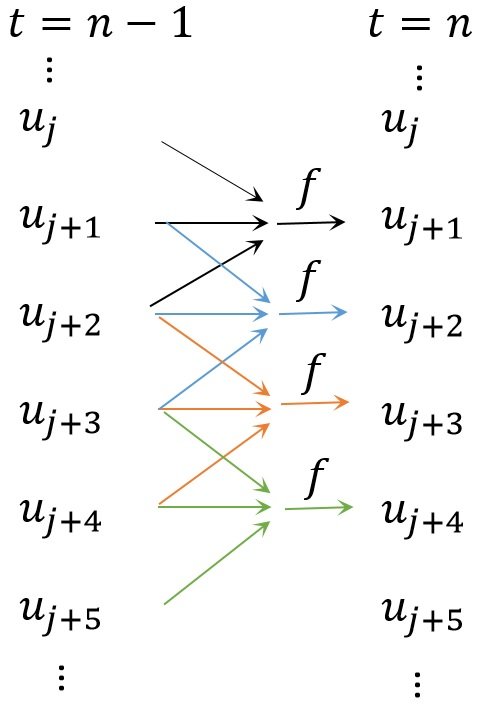
\includegraphics[scale=0.4]{chapterGP/figures/diagram}}
\caption[$f$ as a Local Map] {\label{fig:local map}$f$ as a local map. Here the neighborhood of a site includes itself and two adjacent sites, e.g. $\mathcal{N}(j+1)=\{ j,j+1,j+2 \}$}
\end{figure}

We digress here to give a detailed explanation of the ordering of $\mathcal{N}(j)$, which also exposes the essence of nonparametric methods and biological insight. First, the size of the local neighborhood should reflect the scale of biological iterations in a time step. From a modeling point of view, it is important to determine the size of the local neighborhood, i.e., how many neighbor sites should be included. In other words, we need perform variable selection. Luckily, GP regression with the squared exponential covariance function has built-in variable selection capability, also known as automatic relevance determination \citep{neal2012bayesian,williams1996gaussian,Rasmussen2006}. Second, the ordering of the neighborhood set should be chosen carefully. A straightforward approach would be taking the ordering same as the one of the spatial grids. However, it is beneficial to use an ordering of $\mathcal{N}(j)$ that makes biological sense or exploits certain symmetry of the problem (see next section for a comparison between the naive ordering and a biologically meaningful ordering). In the case of predicting cancer cell invasion, we imagine that the fate of a cell is solely determined by crowdedness of the site it occupies and its immediate neighbor sites. Our data tells us how the cell behaves in a variety of situations of local crowdedness. When we need to make a prediction in a new situation, it is natural to base the prediction on the situations we have seen before. This entails a measure of how similar the new situation is compared to the known situation offered by data. It is straightforward to compare the crowdedness of the occupied site directly by looking their difference. But how about the neighbor sites? We propose an ordering in which the neighbor sites are ranked by its cell density and then take the difference component-wisely. This proposed ordering would further enhance the data efficiency. The price is that it is incapable to capture a process that exhibits advection or anisotropic diffusion. 

We also comment that the notation of $f$ is slightly abused since $f$ was used to denote the global map in (\ref{eq:un=00003Df(un-1)}) while it also presents a local map (Figure \ref{fig:local map}); we will not distinguish them henceforth as it is easily understood in a context. We place a GP prior on $f$, i.e., $f(\mathbf{s})\sim\mathcal{GP}(\mu(\mathbf{s}),k(\mathbf{s},\mathbf{s}'))$. We could use a priori beliefs of the dynamics to specify the mean function $\mu(\cdot)$. For the time being, we simply assume $\mu(u_{\mathcal{N}(j)})=u_{j}$, e.g, the tumor activity stays unchanged, to demonstrate the capability of the method without any specific knowledge of the dynamics. We use the squared exponential covariance function, i.e., 
\begin{equation}
k(\mathbf{s},\mathbf{s}';\boldsymbol{\Lambda}^{-1})=\sigma_{k}^{2}\exp(-\frac{1}{2}(\mathbf{s-s}')^{T}\boldsymbol{\Lambda}^{-1}(\mathbf{s-s}')) \label{eq:cov fun}
\end{equation}
 where $\boldsymbol{\Lambda}=\text{diag}(\ell_{i})$ is a diagonal matrix of the length scales. Here $\ell_{i}$ , $\sigma_{k}$, and possibly $\sigma_{\epsilon}$, are hyperparameters and estimated by maximizing ``marginal likelihood'' \citep{Rasmussen2006}. It should be noted that the choice of covariance function (\ref{eq:cov fun}) is made to facilitate the uncertainty propagation, which will be described later. Another benefit is that the squared exponential covariance function enables automatic relevance determination: the characteristic length $\ell_{i}$ indicates the relative importance of the corresponding variable. 

In this work, we focus on forecasting and defer filtering and smoothing to future study. We assume that the data ($\mathcal{D}$) are two consecutive exact observations of the latent variable $\mathbf{u}$, e.g., $\mathcal{D}=\{\mathbf{u}^{0},\mathbf{u}^{1}\}$.  Ideally, the two consecutive observations should not be too far separated in time.  The assumption on the small time interval is not needed in a strict sense: presumably the larger time interval would lead to larger interaction neighborhood, which entails a more challenging task of learning a higher dimensional mapping. In the case of brain tumor, the two observations  correspond to diagnostic and presurgical imaging which are oftentimes separated by a week or two.  It should also be noted that (\ref{eq:un=00003Df(un-1)}) may lead to negative $\mathbf{u}$ due to the additive Gaussian noise. So we cannot strictly interpret $\mathbf{u}$ as cell density. Instead we understand it as a measure of abundance of cancer cells. We could exponentiate $\mathbf{u}$ and use it as the parameter for Poisson observation model so that we can regain positivity. This approach has been adopted in \citep{Hooten2008}.

To do multi-step forecasting, one simply applies $f$ repeatedly. GP is a non-parametric method, besides a few hyper parameters determined by training data. That is, the training data is needed for every time $f$ is evaluated. Recall that $\mathbf{u}^{2}=f(\mathbf{u}^{1})+\epsilon$ so that $\mathbf{u}^{2}\vert\mathbf{u}^{1}$ is a multivariate normal whose mean and variance are readily known by standard GP regression (see (\ref{eq:f|f*})). To move forward in time, we can apply the same inferences again with test input being $\mathbf{u}^{2}$ to predict $\mathbf{u}^3$. Since $\mathbf{u}^{2}$ is not deterministic and has uncertainty in itself, we need a way to do the same inference with uncertain test input. Fortunately, the mean and variance of $\mathbf{u}^{2}$ can be worked out analytically due to our choice of $k(\mathbf{s},\mathbf{s}')$ and the fact that the product of Gaussian functions is also a Gaussian function (see (\ref{eq:E(u)}), (\ref{eq:cov(u)})). Even though $\mathbf{u}^{2}$ is not necessary normally distributed, we approximate it as a multivariate Gaussian by matching the first two moments. This is a major assumption we make in order to simplify computation. In this way, we can repeat the procedure to propagate the uncertainty. The details on how to take into account the uncertainty of test input are given in the appendix.

One more approximation is necessary when the number of states (grid points) is large. Because the size of the covariance matrix grows quadratically with the number of the states, it quickly becomes impractical to keep track of a dense covariance matrix. For instance, 100 by 100 grids entails a covariance matrix of $10^{8}$ entries. Since we believe that system dynamics is dominated by local interactions, we approximate the dense covariance matrix by only keeping track of the covariance between states which are in a local neighborhood, effectively making the covariance matrix sparse. Similar approaches have been taken in local Kalman Filters \citep{Hunt2007}.


\section{Results} \label{sec:syn-data}

\subsection{Test on 1D Synthetic Data}
\label{sec:GP1d}
We obtain the synthetic data motivated by the discretization of 1D bistable equation
\begin{equation}
u_{j}^{n+1}=u_{j}^{n}+\theta_{1}(u_{j+1}^{n}-2u_{j}^{n}+u_{j-1}^{n})+\theta_{2}u_{j}^{n}(1-u_{j}^{n})(u_{j}^{n}-\alpha)+\epsilon_{j}^{n}\label{eq:synthetic data formula}
\end{equation}
where $\epsilon_{j}^{n}\sim N(0,\sigma^{2})$ is independent in space and time. The choice of (\ref{eq:synthetic data formula}) is due to its simplicity and regularity. The bistable equation is known to have a traveling wave solution given a suitable initial condition. The traveling wave resembles cancer progression. The zero steady state of the homogeneous system is stable. Since the additive white noise inevitably leads to negativity, this stability is favored in contrast to Fisher-KPP equation which may go to negative infinity. Although the slight negativity may pose some issues of interpretability, here $u$ can be interpreted as intensity of underlying tumor activity rather than cell density in a strict sense.           

We use the numerical solution at two consecutive time points as training data. The hyperparameters found by maximizing marginal likelihood are reported in Table \ref{tab:length scales}. It is obvious that only immediate neighbors are relevant and should be included in the neighborhood set. The neighbors that are two sites away have length scale several magnitude larger and hence does not contribute to prediction. It is as expected since the training data are generated from two consecutive time of (\ref{eq:synthetic data formula}).     

Then we obtain our forecasting results and compare them with the observation (a realized sample path). Due to the small chosen $\sigma^2$ and the stability of the traveling wave profile, the observation is considered as the ground truth.  We pick two starting points for forecasting, namely fledged and burgeoning data(see Figures \ref{fig:u subplot ic1} and \ref{fig:u subplot ic2}). Our forecasting predictions captured the general trend of the true process and showed gradual deterioration of the prediction. The quality of the prediction depends on the starting point which controls what the training data is used. Obviously, we shall not expect the forecasting to work well on the region of unseen data. Even though the predicted mean was in disparity with the true mean, the uncertainty bounds were large. This showcases the strength of the method in uncertainty quantification. 

\begin{figure}[ht]
\centerline{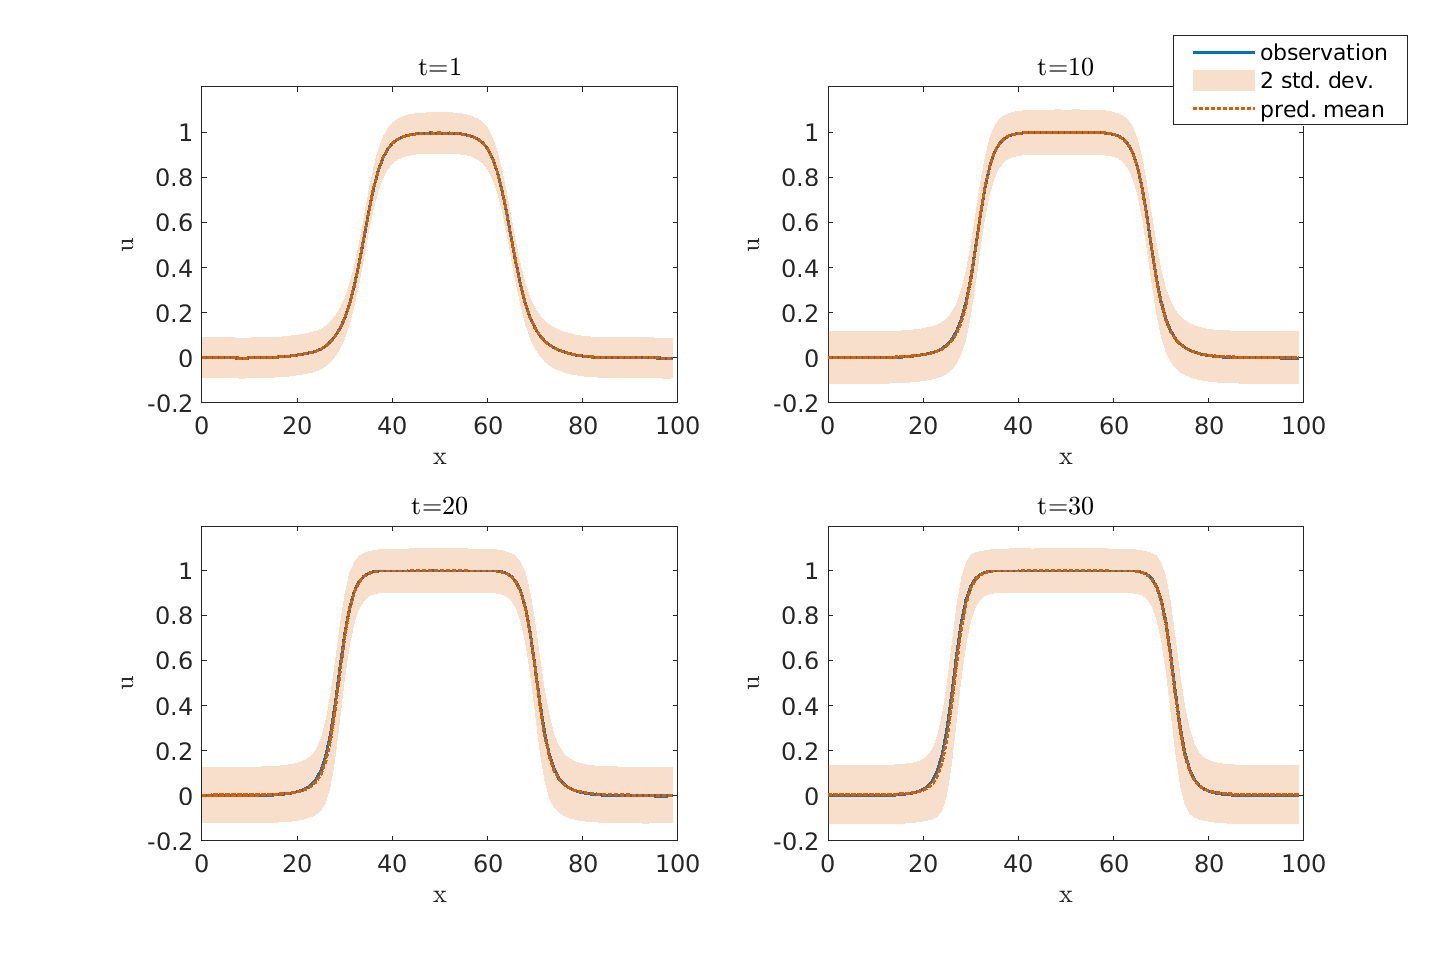
\includegraphics[width=\textwidth]{chapterGP/figures/bistable}}
\caption{\label{fig:u subplot ic1} Forecasting to time $t=2,8,14$ and $20$ with GP trained with fledged synthetic data corrupted with noise $\sigma=0.01$. The shaded bounds indicate the uncertainty (two standard deviation) of the prediction.} 
\end{figure}

\begin{figure}[h]
\centerline{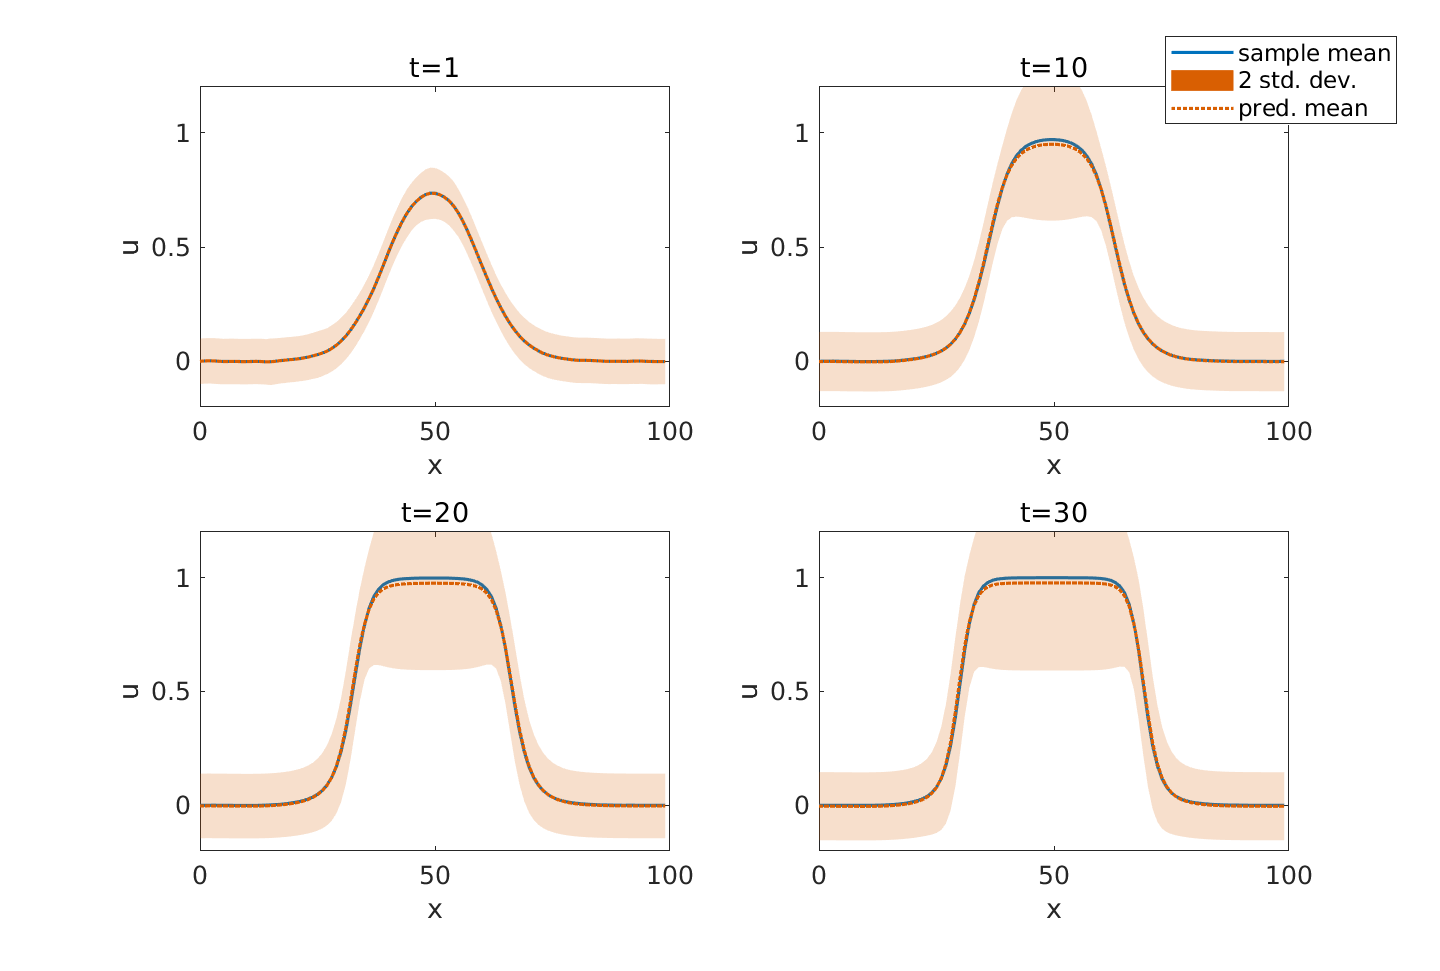
\includegraphics[width=\textwidth]{chapterGP/figures/bistable-short}}
\caption[Forecasting to Time $t=2,8,14$ and $20$ with GP Trained with Unfledged Synthetic Data]{\label{fig:u subplot ic2} Forecasting to time $t=2,8,14$ and $20$ with GP trained with unfledged synthetic data corrupted with noise $\sigma_{\epsilon}=0.01$. The shaded bounds indicate the uncertainty (two standard deviation) of the prediction.}
\end{figure}


The mean squared error (MSE) of the predictive mean and the negative log likelihood (NLL) are summarized in Table \ref{tab:MSE-and-NLL}. Loosely speaking, MSE indicates how good the predictive mean as a point estimate of the ground truth while NLL additionally takes into account the error bound that penalizes being too confident on an inaccurate point estimate or too conservative on an accurate point estimate. We see that biologically meaningful ordering result in smaller MSE and NLL than those obtained by naive ordering (Table \ref{tab:MSE-and-NLL}), meaning that it is a better choice. We also notice that sparse approximation of covariance is prone to be over-confident about the point prediction but overall we are satisfied by its performance. 

\begin{table}[h]
\begin{center}
\caption{Hyperparamters found by maximizing marginal likelihood. The first row has neighborhood size being 3 and the second row has neighborhood size being 5.}
\label{tab:length scales}
\vspace*{12pt}
\begin{tabular}{ccccccc} \hline
 $\sigma_{k}^{2}$ & $\sigma_{\epsilon}^{2}$ & $\ell_{-2}$ & $\ell_{-1}$ & $\ell_{0}$ & $\ell_{1}$ & $\ell_{2}$ \\ \hline
0.1527 & 1.0277e-04 & NA & 6.0574 & 1.5658 & 6.9022 & NA\\ 
0.1527 & 1.0277e-04 & 3.2606e+07 & 6.0574 & 1.5658 & 6.9022 & 3.6812e+07\\ \hline
\end{tabular}
\end{center}
\end{table}


\begin{table}[h]
\begin{center}
\caption[MSE and NLL of GP Forecasting with or without Local Sparse Covariance and Naturally Ordered Neighborhood] {MSE and NLL of GP forecasting with or without local sparse covariance and naturally ordered neighborhood}
\label{tab:MSE-and-NLL}
\vspace*{12pt}
\begin{tabular}{ccccccc} \hline
\multirow{2}{*}{} & \multicolumn{2}{c}{$\sigma_{\epsilon}=0.01$} & \multicolumn{2}{c}{$\sigma_{\epsilon}=0.02$} \\
\cmidrule{2-5} \cmidrule{3-5} \cmidrule{4-5} \cmidrule{5-5} 
 & MSE & NLL & MSE & NLL\\ \hline
sparse ordered & 1.6784e-04 & -306.2233 & 6.3806e-04 & -230.5547 \\
non-sparse ordered & 1.6783e-04 & -340.6569 & 6.3796e-04 & -272.3875 \\
non-sparse non-ordered & 1.8632e-04 & -335.6242 & 6.5192e-04 & -269.7519 \\ \hline
\end{tabular}
\end{center}
\end{table}

\subsection{Test on 2D Synthetic Data}
To get 2D synthetic data, we simply use the 2D version of (\ref{eq:synthetic data formula})
\begin{equation} \label{eq:2d synthetic data formula}
\begin{split}
u_{i,j}^{n+1}  = & u_{i,j}^{n}+\theta_{1}(u_{i+1,j}^{n}+u_{i,j+1}^{n}-4u_{i,j}^{n}+u_{i-,j}^{n}+u_{i,j-1}^{n}) \\
 &+\theta_{2}u_{j}^{n}(1-u_{j}^{n})(u_{j}^{n}-\alpha)+\epsilon_{j}^{n}
\end{split}
\end{equation}
with periodic boundary condition. Same as in section \ref{sec:GP1d}, we use the numerical solution at two consecutive time points as training data. \vphantom{The hyperparameters found by maximizing marginal likelihood are reported in Table ref{tab:2d length scales}.}  It is obvious that only immediate neighbors are relevant and should be included in the neighborhood set. The neighbors that are two sites away have length scale several magnitude larger and hence does not contribute to prediction. Again, this meet our expectation since the data are generated from two consecutive time of (\ref{eq:2d synthetic data formula}).     


In Figure \ref{fig:u subplot 2d}, the prediction over time and its uncertainty is shown. As we can see, the prediction remains regular and its uncertainty gradually grows. The highest uncertainty is at the wave front. The center at $t=20$ shows considerable uncertainty, which is expected since it is the region unseen in training data.    

\begin{figure}[h]
\centerline{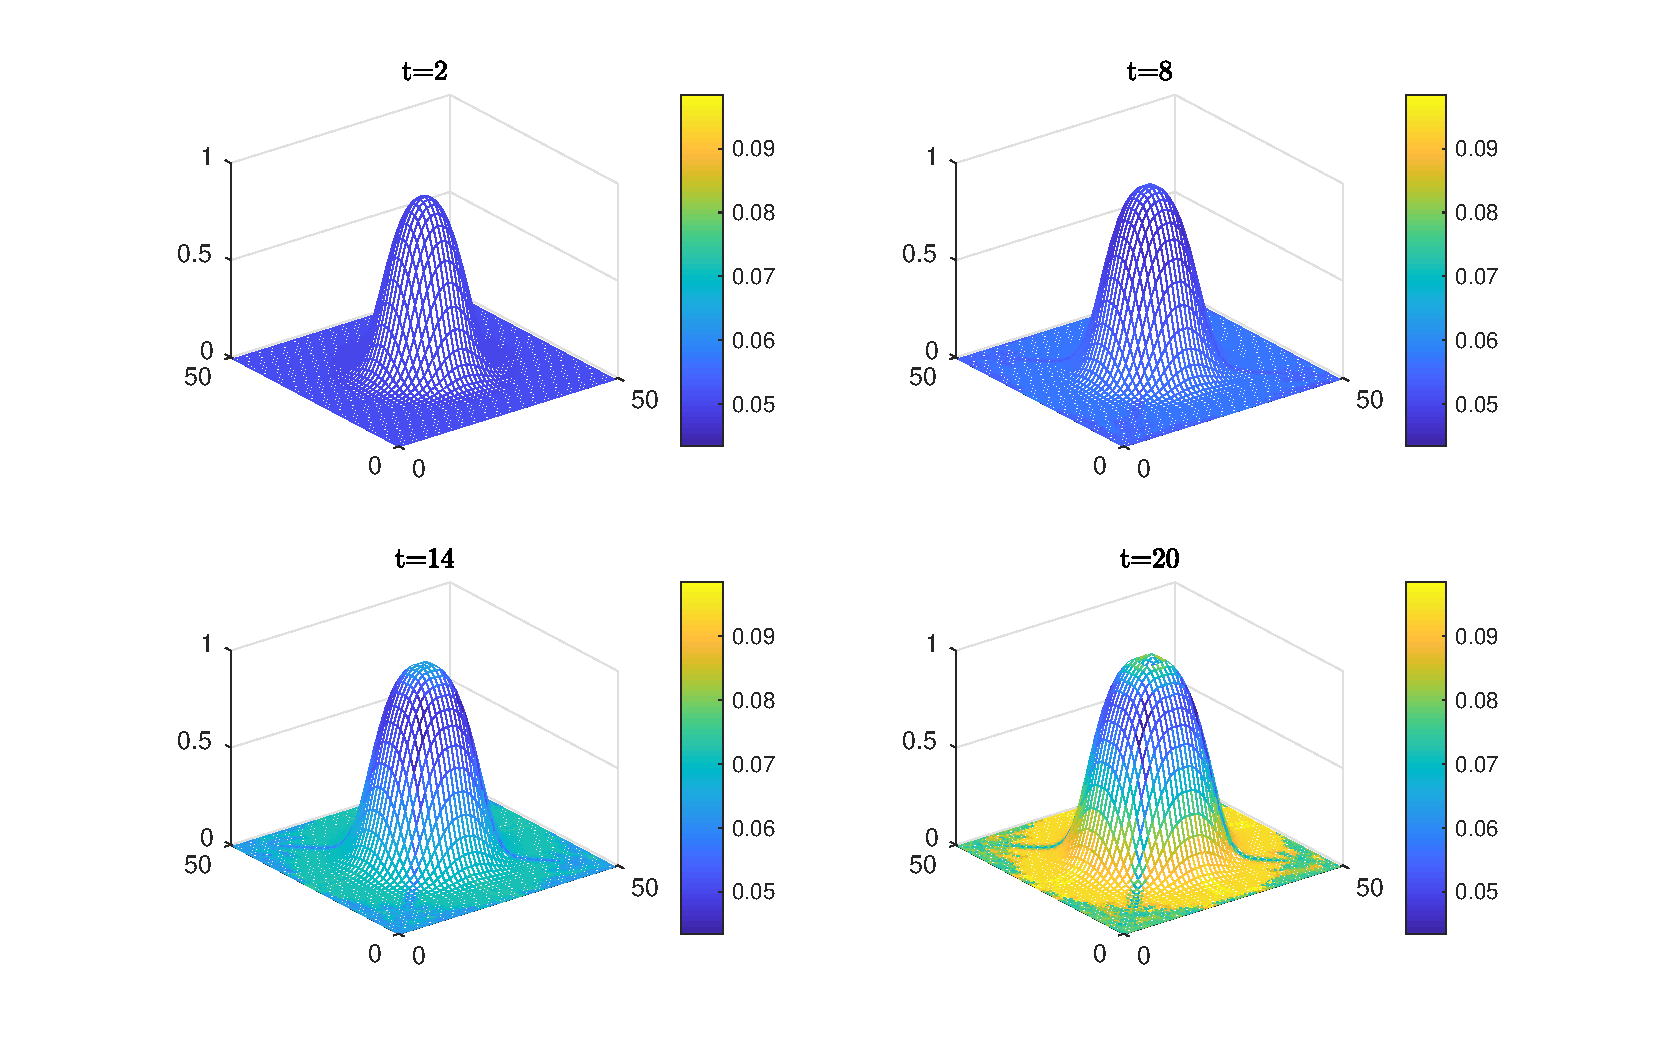
\includegraphics[width=\textwidth]{chapterGP/figures/2d_u_surf_S_color}}
\caption[Forecasting to Time $t=2,8,14$ and $20$ with GP Trained with 2-D Synthetic Data]{\label{fig:u subplot 2d} Forecasting to time $t=2,8,14$ and $20$ with GP trained with 2-D synthetic data corrupted with noise $\sigma_{\epsilon}=0.001$. The colormap indicates the uncertainty (two standard deviation) of the prediction.}
\end{figure}

\subsection{Case Study: Predict Growth of E. coli Colony} 
Modeling of growth of bacterial colony has attracted substantial interests \citep{mimura2000reaction,kawasaki1997modeling,leyva2013effects}. A recent study \citep{he2020predictive} proposed a model of a reaction-diffusion equation with density-dependent diffusion and growth to predict E coli. In that study, greyscale microscopy images were processed and then used for data fitting. Greyscale images are readily suitable for use in the local GP method with minimum processing. So we demonstrate a case study on forecasting growth of E. coli colony.

Data used here consist of microscopy images of an E. coli colony expanding on semi-hard agar medium taken at 2-hour intervals. The images are in greyscale with a numeric value at each pixel indicating its darkness. The images taken at $t=24$ and 26 hours after inoculation are used as training data. The raw images are cropped  according to the one taken at $t=24$ in order to focus on the bacterial colony while allowing enough margin to observe growth. After the images are scaled to a size of 100 by 100 pixels, the interaction neighborhood is reasonably assumed to consist of only immediate neighbors. No further processing of the images are necessary although the raw images themselves are obviously noisy. However, it is one of the purposes of this case study to examine whether the local GP method is able to differentiate real mechanisms from random noise.

The forecasting results in comparison to the real data are shown in Figure \ref{fig:ecoli}. The forecasting in general captures the expansion of the colony and the darkening of the colony center. The expansion of the colony seems to be underestimated. Moreover, the GP method learned artifacts from the training data. For example, the shadow below the colony gets darker in the forecast and the boundary at the top right corner gets brighter. It is not a surprise that these artifacts are amplified since they are systematic patterns in the training data. Hence the GP method is not able to distinguish them from the real pattern presented in the data. The caveat is that care should be given when using the GP method. Researchers with domain knowledge should intervene in cases like this with remedies such as improving data quality. It should be noted that the variance of of the prediction is growing fast in this case, which suggests that the predicted mean should be interpreted with extra caution.          


\begin{figure}[h]
\centerline{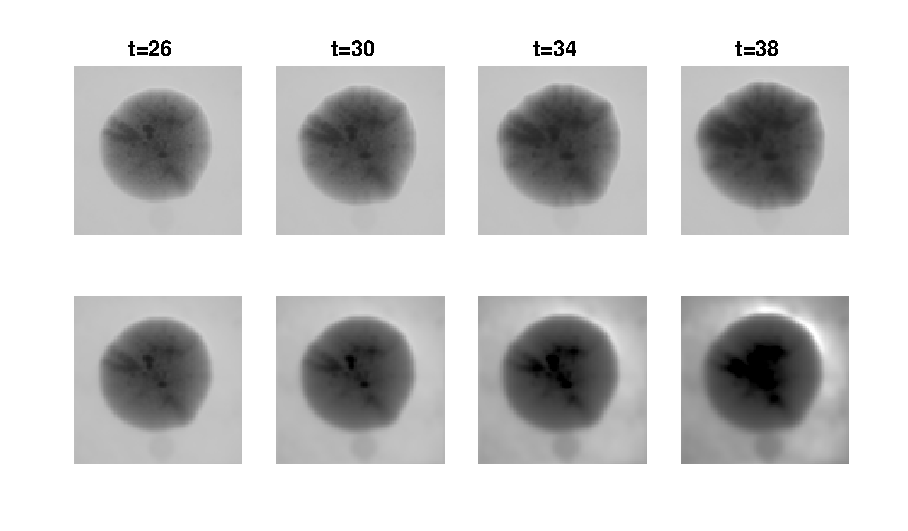
\includegraphics[width=\textwidth]{chapterGP/figures/ecoli100by100}}
\caption[]{\label{fig:ecoli} Forecasts (bottom pane) and real data (top pane) of E. coli colony evolution. The model was trained on the image data obtained at time $t=22$ and 24 hours after inoculation. The forecasts capture two patterns: the expansion of the colony and darkening of the center. But they also amply the artifacts: brightening of the colony edge at the top right and darkening of a shadow at the center bottom}
\end{figure}


\section{Discussion} \label{sec:GP-conclude}
Our method extends the use of GP to learn transition functions into the spatio-temporal processes. With a focus on biological spatio-temporal processes, our method fills a gap in the field of data-driven model discovery. Similar existing methods using GP are mostly about time series modeling on small dimensions \citep{Roberts2013}. The challenge of high dimensionality is circumvented by recognizing the local nature of the spatio-temporal process.

In summary, our method has the following desired features:

First, it replies on minimal assumptions on model building. Instead of formulating a model for the evolution of a biological spatio-temporal process, we take an equation-free approach using GP. In comparison to data-driven model discovering using sparse regression, our method does not require a pre-selected library of candidate terms.

Second, it excels in small-data scenario. By exploiting the local nature of biological spatio-temporal processes, it achieves improved data efficiency so that very sparse time-series data is enough to make predictions. In other words, a local mapping with an input of a few dimensions is learned from the data instead of a global mapping on high dimensional spaces. This improvement of data efficiency has the advantage in applications to predict brain tumor growth for which there are oftentimes only a few brain images of each patient. Data efficiency can be further improved if we order the neighborhood properly with reasonable assumptions. However, this often comes at a price of generality, e.g., ignoring possibility of anisotropic diffusion or advection.   

Third, it has built-in quantification of uncertainty and easy to implement. The advantage of using GP is that posterior variance is readily available for forecasting so that uncertainty in its prediction is naturally quantified. The ease of propagating uncertainty is due to our choice of the squared exponential covariance function for which integration can be done analytically (see Appendix). Hence the propagation of uncertainty is simply done by repeatedly applying the formula \ref{eq:E(u)} and (\ref{eq:cov(u)}), in contrast to ensemble methods and Bayesian methods, which reply on computer simulations \citep{lipkova2019personalized,Kostelich2011a}.   

Last but not least, it reveals a key insight of biological spatio-temporal processes.  This choice of covariance function also makes variable selection easy due to automatic relevance determination. From the selected variables, we can determine the neighborhood size. In the tested cases, our method correctly indicated the relevant variables. Being able to identifying the neighborhood size has biological significance since it tells the scales of spatial interaction in a time step. In the tested cases, the selected neighborhood is symmetric about its center due to the specific choice of the data-generating model. However, it should be noted that this is not necessary the case in practice. A asymmetric shape of a selected neighborhood can be an indicator of anisotropic diffusion or advection of the underlying process. In this sense, our method offers biological interpretation and is different from other black-box machine learning approaches. 

The local GP method in its current form also has limitations. We give a brief discussion below and point out future directions.         

Even though automatic relevance determination correctly identified relevant variables in the case of synthetic data. But it only gives a relative importance between variables. It is foreseeable that in the case of real-world data, the cut-off of relevance will not be so clear. Ideally, we need a more informed variable selection criterion with a built-in cut-off. This will be one of the directions of future studies. 

We left out the observation model in this paper. An observation model is needed to solve more realistic problems because exact observation is rarely available in practice. It is important to extend the local GP method to put it in the state space modeling framework. As noted in our testing results, the prediction deteriorates over time and thus there is need to incorporate new data to correct predictions as they become available. In other words, we need a filtering algorithm which can assimilate data in an iterative fashion similar to Kalman filters or particle filters. This shall be the focus of future study. It should be noted that state space modeling is challenging for nonparametric methods because of loss of Markov property in (\ref{eq:un=00003Df(un-1)}) (note that $f(\cdot)$ itself depends on all historical $\mathbf{u}$.) There are some attempts aimed at resolving this issue \citep{frigola2013bayesian,Ghosh2014} but it is not immediately clear how these can be extended to a high-dimensional spatio-temperoal process. 

We approximated the state variables for all subsequent forecasting with normal distributions. This approximation leads to computationally efficiency as the work required to propagate uncertainty is done via a reasonable amount of matrix algebra and computation (See Appendix). The error introduced and whether there are computational alternatives are also left for future investigation.

Another approximation we used to achieve the sparsity of the covariance matrix can also introduce error. The approximation is justified if the the covariance between remote sites decay rapidly. Since spatial independent noise is added in each time step, the assumption is expected to be met at least in the long term. A rigorous error analysis await for future studies. It should be pointed out that similar practice and rationale have been adopted in local Kalman filters and local particle filters. The localization of a Kalman filter makes parallelization of computation possible \citep{ott2004local,Hunt2007,szunyogh2008local}. Moreover, it is believed that local analysis avoids spurious correlation that would otherwise allow obervation at one location to influence the analysis of a  location an arbitrarily large distance away \citep{Hunt2007}. It should be noted that in our case the correlation between remote sites are not necessarily spurious because of the nonparametric nature of the method. \cite{Rebeschini2015} gave a rigorous proof to justify a simple locality implementation called block particle filters. Since then, the local particle filter has been implemented by \cite{morzfeld2018variational,farchi2018comparison}. These ideas lead to some clues to further develop the local GP method.     


\section{Conclusion}
We proposed a method to learn biological dynamics from spatio-temporal data by Gaussian processes.  Instead of formulating a mathematical model for the process,  the transition function is learned from data by GP. By exploiting the local nature of the dynamics, we improved the data efficiency and solved the problem of sparsity of temporal data. By exploiting Gaussianity, prediction and uncertainty can be propagated in a computationally efficient way. As shown in the test cases, this method not only excels at forecasting with quantified uncertainty but also generates insights to the underlying process. Recognizing its potential and current limitation, we pointed out directions of future studies. 


%\begin{acknowledgements}
%If you'd like to thank anyone, place your comments here
%and remove the percent signs.
%\end{acknowledgements}


% Authors must disclose all relationships or interests that 
% could have direct or potential influence or impart bias on 
% the work: 
%
% \section*{Conflict of interest}
%
% The authors declare that they have no conflict of interest.


% BibTeX users please use one of
\bibliographystyle{spbasic}      % basic style, author-year citations
%\bibliographystyle{spmpsci}      % mathematics and physical sciences
%\bibliographystyle{spphys}       % APS-like style for physics
\bibliography{ref2}   % name your BibTeX data base

\newpage
\section*{Appendix: Derivation of Prediction and Uncertainty Propagation} \label{app:prop-uncertainty}
Since product of Gaussian functions are again a Gaussian, we can do the following integration analytically. In general, for $\mathbf{x}\sim N(\boldsymbol{\mu},\boldsymbol{\Sigma})$
\begin{align}
 & \int k(\hat{\mathbf{x}},\mathbf{x};\mathbf{V})p(\mathbf{x})d\mathbf{x}\nonumber \\
= & \sigma_{k}^{2}\left|\boldsymbol{\Sigma}\mathbf{V}+\mathbf{I}\right|^{-1/2}\exp\bigg(-\frac{1}{2}(\hat{\mathbf{x}}-\boldsymbol{\mu})^{T}(\boldsymbol{\Sigma}+\mathbf{V}^{-1})^{-1}(\hat{\mathbf{x}}-\boldsymbol{\mu})\bigg)\label{eq:int kp}
\end{align}
\begin{align}
 & \int k(\hat{\mathbf{x}},\mathbf{x};\mathbf{V})k(\hat{\mathbf{y}},\mathbf{x};\mathbf{W})p(\mathbf{x})d\mathbf{x}\nonumber \\
= & \frac{\sigma_{k}^{4}}{\left|\boldsymbol{\Sigma}(\mathbf{V}+\mathbf{W})+\mathbf{I}\right|^{1/2}}\exp\bigg(-\frac{1}{2}\big(\hat{\mathbf{x}}^{T}\mathbf{V}\hat{\mathbf{x}}+\hat{\mathbf{y}}\mathbf{W}\hat{\mathbf{y}}-\mathbf{q}^{T}(\mathbf{V}+\mathbf{W})\mathbf{q}\big)\bigg)\nonumber \\
 & \exp\bigg(-\frac{1}{2}(\mathbf{q}-\boldsymbol{\mu})^{T}(\boldsymbol{\Sigma}+(\mathbf{V}+\mathbf{W})^{-1})^{-1}(\mathbf{q}-\boldsymbol{\mu})\bigg)\label{eq:int k k p}
\end{align}
where $\mathbf{q}=(\mathbf{V}+\mathbf{W})^{-1}(\mathbf{V}\hat{\mathbf{x}}+\mathbf{W}\hat{\mathbf{y}})$. In the following, we show how to take into account of the uncertainty of input in forecasting by using (\ref{eq:int kp}) and (\ref{eq:int k k p}). 

To simplify notations, we denote training data as $\mathcal{D}=(\hat{\mathbf{u}},\tilde{\mathbf{v}})$ and test input $\mathbf{u}^{*}\sim N(\mathbf{m},\mathbf{S})$. Note that here we deviate from our previous notations in main text in favor of presenting a general method. We want to find the mean and variance of the test output $\mathbf{u}\equiv(u_{j})_{j\in\{1:n_{x}\}}$. The GP regression tells that 
\[
\mathbf{u}\vert\mathbf{u}^{*},\mathcal{D}\sim N(\mathbf{u}^{*}+\mathbf{K}_{*}^{T}\mathbf{\boldsymbol{\Sigma}}^{-1}(\tilde{\mathbf{v}}-\hat{\mathbf{u}}),\mathbf{K}_{**}-\mathbf{K}_{*}^{T}\mathbf{\boldsymbol{\Sigma}}^{-1}\mathbf{K}_{*})
\]
where $(\mathbf{K}_{*})_{ij}=k(\hat{\mathbf{u}}_{i-1:i+1},\mathbf{u}_{j-1:j+1}^{*})$, $(\mathbf{\Sigma})_{ij}=k(\hat{\mathbf{u}}_{i-1:i+1},\hat{\mathbf{u}}_{j-1:j+1})+\sigma_{\epsilon}^{2}\delta_{ij}$ and $(\mathbf{K}_{**})_{ij}=k(\mathbf{u}_{i-1:i+1}^{*},\mathbf{u}_{j-1:j+1}^{*})$. To simplify notation we let $\boldsymbol{\beta}=\boldsymbol{\Sigma}^{-1}(\tilde{\mathbf{v}}-\hat{\mathbf{u}})$ and note that it is sorely determined by training data $\mathcal{D}$. The mean of $\mathbf{u}$ is easy, i.e., 
\begin{align}
E[\mathbf{u}] = & E[E[\mathbf{u}\vert\mathbf{u}^{*}]] \nonumber \\
 = & E[\mathbf{u}^{*}+\mathbf{K}_{*}^{T}\boldsymbol{\beta}] \nonumber \\
 = & \mathbf{m}+\mathbf{L}^{T}\boldsymbol{\beta}\label{eq:E(u)}
\end{align}
where by simply applying (\ref{eq:int kp}), we have
\begin{eqnarray*}
(\mathbf{L})_{rj} & = & \int k(\hat{\mathbf{u}}_{r-1:r+1},\mathbf{u}_{j-1:j+1}^{*};\boldsymbol{\Lambda}^{-1})p(\mathbf{u}_{j-1:j+1}^{*})d\mathbf{u}_{j-1:j+1}^{*} \\
 & = & \sigma_{k}^{2}\left|\mathbf{S}_{\mathcal{N}(j)}\mathbf{\Lambda}^{-1}+\mathbf{I}\right|^{-1/2} \\
 & & \exp\bigg(-\frac{1}{2}(\hat{\mathbf{u}}_{r-1:r+1}-\mathbf{m}_{j-1:j+1})^{T}(\mathbf{S}_{b_{j}}+\mathbf{\Lambda})^{-1}(\hat{\mathbf{u}}_{r-1:r+1}-\mathbf{m}_{j-1:j+1})\bigg) 
\end{eqnarray*}
where $\mathbf{S}_{\mathcal{N}(j)}$ is the sub-covariance matrix that concerns only $\mathcal{N}(j)$.

The variance-covariance matrix of $\mathbf{u}$ is slightly more complicated. Let's consider it component-wisely. By law of total variance, 
\begin{eqnarray*}
cov(u_{i},u_{j}) & = & E[cov(u_{i},u_{j}\vert\mathbf{u}^{*})]+cov(E[u_{i}\vert\mathbf{u}^{*}],E[u_{j}\vert\mathbf{u}^{*}])
\end{eqnarray*}
We first compute 
\begin{align*}
 & cov(E[u_{i}\vert\mathbf{u}^{*}],E[u_{j}\vert\mathbf{u}^{*}])\\
= & E[E[u_{i}\vert\mathbf{u}^{*}]E[u_{j}\vert\mathbf{u}^{*}]]-E[E[u_{i}\vert\mathbf{u}^{*}]]\cdot E[E[u_{j}\vert\mathbf{u}^{*}]]\\
= & E[(u_{i}^{*}+\mathbf{k}_{*i}^{T}\boldsymbol{\beta})(u_{j}^{*}+\mathbf{k}_{*j}^{T}\boldsymbol{\beta})]-(m_{i}+\mathbf{l}_{i}^{T}\boldsymbol{\beta})(m_{j}+\mathbf{l}_{j}^{T}\boldsymbol{\beta})\\
= & E[u_{i}^{*}u_{j}^{*}]+E[u_{i}^{*}\mathbf{k}_{*j}^{T}\boldsymbol{\beta}]+E[\mathbf{k}_{*i}^{T}\boldsymbol{\beta}u_{j}^{*}]+\boldsymbol{\beta}^{T}E[\mathbf{k}_{*i}\mathbf{k}_{*j}^{T}]\boldsymbol{\beta}-(m_{i}+\mathbf{l}_{i}^{T}\boldsymbol{\beta})(m_{j}+\mathbf{l}_{j}^{T}\boldsymbol{\beta})\\
= & S_{ij}+E[u_{i}^{*}\mathbf{k}_{*j}^{T}\boldsymbol{\beta}]+E[\mathbf{k}_{*i}^{T}\boldsymbol{\beta}u_{j}^{*}]+\boldsymbol{\beta}^{T}(E[\mathbf{k}_{*i}\mathbf{k}_{*j}^{T}]-\mathbf{l}_{i}\mathbf{l}_{j}^{T})\boldsymbol{\beta}-(m_{i}\mathbf{l}_{j}^{T}+m_{j}\mathbf{l}_{i}^{T})\boldsymbol{\beta}
\end{align*}
where $\mathbf{k}_{*i}$ is the i-th column of $\mathbf{K}_{*}$ and $\mathbf{l}_{i}$ is the i-th column of $\mathbf{L}$. We try to determine term by term. First, 
\[
E[u_{i}^{*}u_{j}^{*}]=S_{ij}+m_{i}m_{j}.
\]

Second and third, $E[u_{i}^{*}\mathbf{k}_{*j}^{T}]$ is a vector and its r-th entry is 
\begin{align*}
 & \int u_{i}^{*}k(\hat{\mathbf{u}}_{\mathcal{N}(r)},\mathbf{u}_{\mathcal{N}(j)}^{*})p(\mathbf{u}_{\mathcal{N}(j)\cup i}^{*})d\mathbf{u}_{\mathcal{N}(j)\cup i}^{*}\\
= & \int u_{i}^{*}k(\mathbf{P}^{T}\hat{\mathbf{u}}_{\mathcal{N}(r)},\mathbf{u}_{\mathcal{N}(j)\cup i}^{*};\mathbf{P}^{T}\boldsymbol{\Lambda}^{-1}\mathbf{P})p(\mathbf{u}_{\mathcal{N}(j)\cup i}^{*})d\mathbf{u}_{\mathcal{N}(j)\cup i}^{*}\\
= & \text{last entry of }(\mathbf{P}^{T}\boldsymbol{\Lambda}^{-1}\mathbf{P}+\mathbf{S}_{\mathcal{N}(j)\cup i}^{-1})^{-1}(\mathbf{P}^{T}\boldsymbol{\Lambda}^{-1}\hat{\mathbf{u}}_{r-1:r+1}+\mathbf{S}_{\mathcal{N}(j)\cup i}^{-1}\mathbf{m}_{\mathcal{N}(j)\cup i\cup i})
\end{align*}
if $i\notin\mathcal{N}(j)$ where $\mathbf{P}\mathbf{u}_{\mathcal{N}(j)\cup i}^{*}=\mathbf{u}_{\mathcal{N}(j)}^{*}$. If $i\in\mathcal{N}(j)$, the r-th entry of $E[u_{i}^{*}\mathbf{k}_{*j}^{T}]$ is the one of the entries of 
\[
(\boldsymbol{\Lambda}^{-1}+\mathbf{S}_{\mathcal{N}(j)}^{-1})^{-1}(\boldsymbol{\Lambda}^{-1}\hat{\mathbf{u}}_{\mathcal{N}(r)}+\mathbf{S}_{\mathcal{N}(j)}^{-1}\mathbf{m}_{\mathcal{N}(j)})
\]
 that corresponds to the position of $i$ in $\mathcal{N}(j)$.

Fourth, $E[\mathbf{k}_{*i}\mathbf{k}_{*j}^{T}]\equiv\tilde{\mathbf{L}}$ is a matrix with 
\begin{eqnarray*}
\tilde{L}_{rs} & = & \int k(\hat{\mathbf{u}}_{\mathcal{N}(r)},\mathbf{u}_{\mathcal{N}(i)}^{*})k(\hat{\mathbf{u}}_{\mathcal{N}(s)},\mathbf{u}_{\mathcal{N}(j)}^{*})p(\mathbf{u}_{\mathcal{N}(i)\cup\mathcal{N}(j)}^{*})d\mathbf{u}_{\mathcal{N}(i)\cup\mathcal{N}(j)}^{*}\\
 & = & \int k(\mathbf{P}^{T}\hat{\mathbf{u}}_{\mathcal{N}(r)},\mathbf{u}_{\mathcal{N}(i)\cup\mathcal{N}(j)}^{*};\mathbf{P}^{T}\boldsymbol{\Lambda}^{-1}\mathbf{P})k(\mathbf{Q}^{T}\hat{\mathbf{u}}_{\mathcal{N}(s)},\mathbf{u}_{\mathcal{N}(i)\cup\mathcal{N}(j)}^{*};\mathbf{Q}^{T}\boldsymbol{\Lambda}^{-1}\mathbf{Q})\\
 & & p(\mathbf{u}_{\mathcal{N}(i)\cup\mathcal{N}(j)}^{*})d\mathbf{u}_{\mathcal{N}(i)\cup\mathcal{N}(j)}^{*}
\end{eqnarray*}
where $\mathbf{P}\mathbf{u}_{\mathcal{N}(i)\cup\mathcal{N}(j)}^{*}=\mathbf{u}_{\mathcal{N}(i)}^{*}$ and $\mathbf{Q}\mathbf{u}_{\mathcal{N}(i)\cup\mathcal{N}(j)}^{*}=\mathbf{u}_{\mathcal{N}(j)}^{*}$. We note that the above is in the form of (\ref{eq:int k k p}) and hence can be readily evaluated. 

Next we compute 
\begin{eqnarray*}
E[cov(u_{i},u_{j}\vert\mathbf{u}^{*})] & = & E[k(\mathbf{u}_{i-1:i+1}^{*},\mathbf{u}_{j-1:j+1}^{*})]-E[Tr(\mathbf{\Sigma}^{-1}\mathbf{k}_{*i}\mathbf{k}_{*j}^{T})]
\end{eqnarray*}
The first term on right hand side 
\begin{eqnarray*}
E[k(\mathbf{u}_{\mathcal{N}(i)}^{*},\mathbf{u}_{\mathcal{N}(j)}^{*})] & = & \int k(\mathbf{u}_{\mathcal{N}(i)}^{*},\mathbf{u}_{\mathcal{N}(j)}^{*})p(\mathbf{u}_{\mathcal{N}(i)\cup\mathcal{N}(j)}^{*})d\mathbf{u}_{\mathcal{N}(i)\cup\mathcal{N}(j)}^{*}\\
 & = & \int k(0,\mathbf{u}_{\mathcal{N}(i)\cup\mathcal{N}(j)}^{*};\mathbf{P}^{T}\boldsymbol{\Lambda}^{-1}\mathbf{P})p(\mathbf{u}_{\mathcal{N}(i)\cup\mathcal{N}(j)}^{*})d\mathbf{u}_{\mathcal{N}(i)\cup\mathcal{N}(j)}^{*}
\end{eqnarray*}
where $\mathbf{P}\mathbf{u}_{i-1:i+1\cup j-1:j+1}^{*}=\mathbf{u}_{i-1:i+1}^{*}-\mathbf{u}_{j-1:j+1}^{*}$. The second term
\begin{eqnarray*}
E[Tr(\mathbf{\Sigma}^{-1}\mathbf{k}_{*i}\mathbf{k}_{*j}^{T})] & = & Tr(\boldsymbol{\Sigma}^{-1}E[\mathbf{k}_{*i}\mathbf{k}_{*j}^{T}])\\
 & = & Tr(\boldsymbol{\Sigma}^{-1}\tilde{\mathbf{L}})
\end{eqnarray*}

Putting together, we have 
\begin{align}
cov(u_{i},u_{j}) & = & S_{ij}+E[u_{i}^{*}\mathbf{k}_{*j}^{T}\boldsymbol{\beta}]+E[\mathbf{k}_{*i}^{T}\boldsymbol{\beta}u_{j}^{*}]+\boldsymbol{\beta}^{T}(E[\mathbf{k}_{*i}\mathbf{k}_{*j}^{T}]-\mathbf{l}_{i}\mathbf{l}_{j}^{T})\boldsymbol{\beta} \nonumber \\
&  & -(m_{i}\mathbf{l}_{j}^{T}+m_{j}\mathbf{l}_{i}^{T})\boldsymbol{\beta} \label{eq:cov(u)}
\end{align}

\end{document}
% end of file template.tex

